% \todo{include refs from FWO proejct in bibtex. I included the files but doubles should be removed until bibtex produces no more errors.}


%Need for explanations of reasoning systems
In the last few years, as AI systems employ more advanced reasoning mechanisms and computation power, it becomes increasingly difficult to understand why certain decisions are made. 
Explainable AI (XAI) research aims to fulfil the need for trustworthy AI systems to understand why the system made a decision for verifying the correctness of the system, as well as to control for biased or systematically unfair decisions.

Explainable AI is often studied in the context of (black box) prediction systems such as neural networks, where the goal is to provide insight into which part(s) of the input is important in the \textit{learned} model. 
These insights (or local approximations thereof) can justify why certain predictions are made. 
In that setting, a range of techniques have been developed, ranging from local explanations of predictions at the \textit{feature level}~\cite{ribeiro2016should,lundberg2017unified} to \textbf{visual explanations} with \textit{saliency maps} \cite{selvaraju2017grad}. %\emilio{Tias, do you mean \cite{selvaraju2017grad}}~\tias{TODO}. 
Adadi et al.~\cite{Adadi_2018}, Guidotti et al.~\cite{guidotti2018survey} and more recently Arrieta et al.~\cite{Barredo_Arrieta_2020}, survey the latest trends and  major research directions in this area.
In contrast, in Constraint Satisfaction Problems (CSP) \cite{fai/Rossi06}, the problem specification is an explicit \textit{model-based representation} of the problem, hence creating the opportunity to explain the inference steps directly in terms of this representation.



% Explainable AI research aims to fulfil the need for trustworthy AI systems that can explain their reasoning in a human-understandable way. 
% As these systems employ more advanced reasoning mechanisms and computation power, it becomes increasingly difficult to understand why certain decisions are made. 
% Understanding the decisions is important for verifying the correctness of the system, as well as to control for biased or systematically unfair decisions.

% Explainable AI is often studied in the context of (black box) machine learning systems such as neural networks, where the goal is to provide insight into what part of the input is important in the \textit{learned} model. These insights (or local approximations thereof) can justify why certain predictions are made. In contrast, in constraint satisfaction problems, the problem specification is an explicit model-based representation of the problem, hence creating the opportunity to explain the inference steps directly in terms of this representation.

Explanations have been investigated in constraint solving before, most notably for explaining overconstrained, and hence unsatisfiable, problems to a user~\cite{junker2001quickxplain}.
Our case is more general in that it also works for satisfiable problems.
At the solving level, in lazy clause generation solvers, explanations of a constraint are studied in the form of an implication of low-level Boolean literals that encode the result of a propagation step of an individual constraint~\cite{feydy2009lazy}. 
Also, no-goods (learned clauses) in conflict-driven clause learning SAT solvers can be seen as explanations of failure during search~\cite{marques2009conflict}. 
These are not meant to be human-interpretable but rather to propagate effectively.

We aim to explain the process of propagation in a constraint solver, independent of the consistency level of the propagation and without augmenting the propagators with explanation capabilities.
For problems that can --- given a strong enough propagation mechanism --- be solved without search, e.g. problems such as logic grid puzzles with a unique solution, this means explaining the entire problem solving process. 
For problems involving search, this means explaining the inference steps  in one search node. 
It deserves to be stressed that we are not interested in the computational cost of performing an expensive form of propagation, but in explaining all consequences of a given assignment to the user in a way that is as understandable as possible. 

More specifically, we aim to develop an explanation-producing system that is complete and interpretable. 
By \emph{complete} we mean that it finds a \emph{sequence} of small reasoning steps that, starting from the given problem specification and a partial solution, derives all consequences. 
Gilpin et al.~\cite{DBLP:conf/dsaa/GilpinBYBSK18} define \emph{interpretable} explanations as ``descriptions that are simple enough for a person to understand, using a vocabulary that is meaningful to the user''. 
Our guiding principle is that of simplicity, where smaller and simpler explanations are better. 

% An open issue when presenting a sequence of explanations is that of the level of abstraction used.
An open issue when presenting a sequence of explanations is the level of abstraction used.
%On top of this idea of explaining propagations by means of as simple as possible steps, we add a mechanism for controlling the level of abstraction of the explanation sequence. 
Starting from a sequence of as-simple-as-possible explanations as we do, there are two ways to change the level of abstraction.
The first direction is that one could \emph{group} multiple single steps into one larger step that can then be expanded on the fly. 
The second direction is to provide a \emph{more detailed} explanation of harder steps which can not be broken into simpler steps with the standard mechanism.
While the first direction can be useful when explanations get very long, from a theoretical perspective, it is less interesting. 
The second direction on the other hand is interesting for several reasons. First of all, we noticed that some of the generated steps are still too complicated to be understood easily and thus really require being explained in more detailed. Secondly, breaking them up in smaller steps is an interesting challenge. Indeed, since we start from the idea that steps should be as simple as possible, it should not be possible to break them up further. 
To still break them up further, we took inspiration from methods people use when solving puzzles, and mathematicians use when proving theorems. 
That is, for explaining a single step in more detail we work using reasoning by contradiction: starting from the negation of a consequence, we explain how a contradiction is obtained.  In essence, we assume the negation of the derived fact, and can then reuse the principle of explanation steps to construct a sequence that leads to an inconsistency. 
This novel approach allows us to provide a mechanism for \emph{zooming in} on the most difficult explanation step.

In practice, we choose to present the constraints in natural language, which is an obvious choice for logic grid puzzles as they are given in the form of natural language \textit{clues}. 
We represent the previously and newly derived facts visually, as can be seen in the grid in Figure~\ref{fig:zebrascreen}. In this figure, the implicit ``Bijectivity'' axiom present in each logic grid puzzle is used to derive the following: since Arrabiata sauce was eaten with Farfalle, it was not eaten with any of the other pasta types.

% \bart{Make better quality screenshot! Also check the others. }
\begin{figure}[ht]
\centering
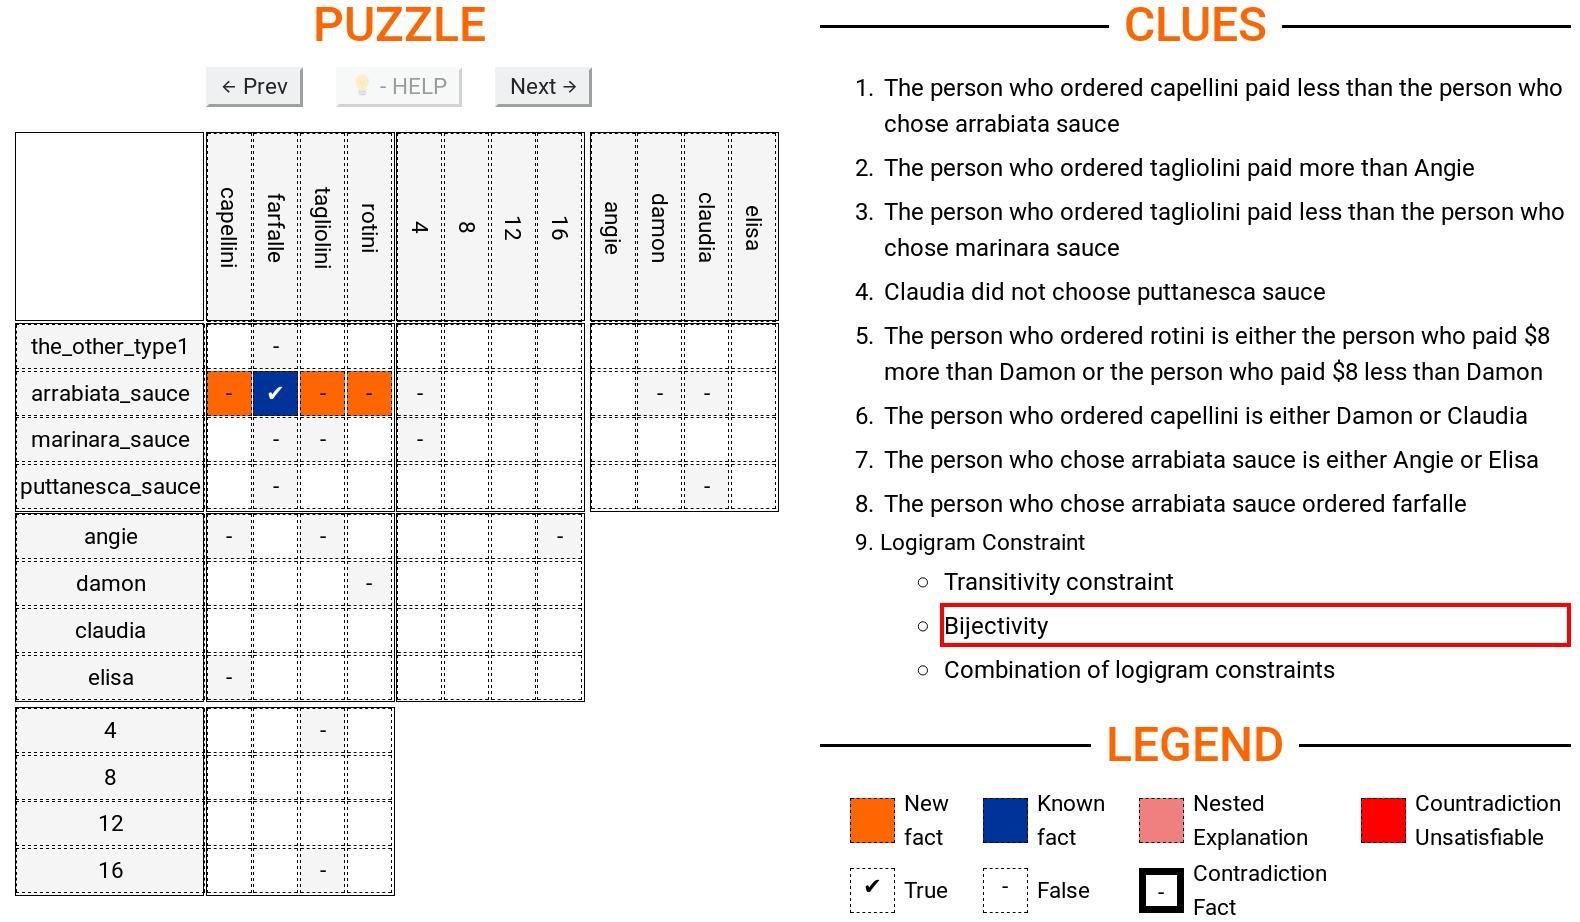
\includegraphics[width=0.9\linewidth]{figures/introduction.jpeg}
\caption{Demonstration of explanation visualisation.}
\label{fig:zebrascreen}
\end{figure}

%HolyGrail challenge and related work
Our work and more specifically the use case of logic grid puzzles is motivated by the ``Holy Grail Challenge''\footnote{\url{https://freuder.wordpress.com/pthg-19-the- third-workshop-on-progress-towards-the-holy-grail/}} which had as objective to provide \textit{automated} processing of logic grid puzzles, ranging from natural language processing, to solving, and explaining.
% An earlier version of our system won the challenge at the workshop. 
% \emilio{do we really need to say that ?}\bart{What? The line in comment about winning above? Not really, no}
While our integrated system, \ourtool, has the capability of solving logic grid puzzle starting from the natural language clues (see Section \ref{sec:holistic}), the focus in this paper is on the explanation-producing part of the system.

The explanation-generating techniques we develop can be applied in a multitude of use cases. 
For instance, it can explain the entire sequence of reasoning, such that a user can better understand it, or in case of an unexpected outcome can debug the reasoning system or the set of constraints that specify the problem. 
As our approach starts from an arbitrary set of facts, it can also be used as a virtual assistant when a user is stuck in solving a problem.
The system will explain the simplest possible next step, or in an interactive setting, the system can explain how it would complete a partial solution of a user. Such explanations can be useful in the context of  \emph{interactive configuration} \cite{felfernig2014knowledge} where a domain expert solves a problem (e.g., a complicated scheduling or rostering problem) but is assisted by an intelligent system. 
The system in that case typically does not have the all the knowledge required to solve the problem since certain things are hard to formalize, especially when personal matters are involved. In such case, the system cannot find the optimal solution automatically, but it can help the expert for instance by propagating information that follows from its knowledge base. In case something undesired is propagated, the user might need an explanation about \emph{why} this follows; this is where our methods can be plugged in.
% 
% 
Finally, our measures of simplicity of reasoning steps can be used to estimate the difficulty of solving a problem for a human, e.g. for gradual training of experts.
% % \bart{Mention interactive configuration here as an application domain? }

% As far as industrial 
% Finally, as we will allow users to \textbf{explore} the solution space \textbf{interactively}, there is a strong link to. We believe our notions of explanation will prove to be valuable there as well, to allow more transparent guidance of the user to good solutions. 

Summarized, our main contributions are the following:
\begin{itemize}
	\item We formalize the problem of step-wise explaining the propagation of a constraint solver through a sequence of small inference steps;
	\item We propose an algorithm that is agnostic to the propagators and the consistency level used, and that can provide explanations for inference steps involving arbitrary combinations of constraints;
	\item Given a cost function quantifying human interpretability, our method uses an optimistic estimate of this function to guide the search to low-cost explanations, thereby making use of Minimal Unsatisfiable Subset extraction;
	\item We introduce nested explanations to provide additional explanations of complex inference steps using reasoning by contradiction;
	\item We experimentally demonstrate the quality and feasibility of the approach in the domain of logic grid puzzles.
\end{itemize}


This paper is structured as follows. In Section~\ref{sec:related-work}, we discuss related work. Section \ref{sec:background}, explains the rules of logic grid puzzles and presents background information. 
Sections \ref{sec:problem-definition} and \ref{sec:nested-explanation}, formalize the theory of the explanation-production problem on two abstraction levels, while Section \ref{sec:expl-gen-prod} describes the algorithms needed to solve the explanation-production problem.
In Section \ref{sec:zebra}, we motivate our design decisions using observations from the \ourtool use case. 
Section \ref{sec:holistic} describes the entire information pipeline of the \ourtool integrated system. 
In Section \ref{sec:experiments}, we experimentally study the feasibility of our approach. 
Finally, we conclude the paper in Section \ref{sec:conclusion}.


% Publication history
\paragraph{Publication history} This paper is an extension of previous papers presented at workshops and conferences \cite{claesuser,DBLP:conf/bnaic/ClaesBCGG19,ecai/BogaertsGCG20}. The current paper extends the previous papers with more detailed examples, additional experiments, as well as the formalization of what we call \emph{nested explanation sequences}.

% Our nested explanation XAI submission stems from the work originally proposed \cite{ecai/BogaertsGCG20} and motivated by the results from the demonstrator submitted to IJCAI-PRICAI 2020.
